\documentclass{beamer}

\mode<presentation>{
\usepackage{tikz}
\usetheme{JuanLesPins} 
\usepackage{amsmath}
\usepackage{array}
\usecolortheme{dolphin} 
}
\usepackage{graphicx} 
\usepackage{booktabs} 

\title[Project]{EE1390 P2} 
\title{EE1390}
\subtitle{BFSK (Binary Frequency Shift Keying)}
\author{Sai Manasa Pappu EE17BTECH11036 \\
        Raagini Vishnubotla EE17BTECH11050
   } 
\date{IIT Hyderabad, Feb 2019}


\begin{document}


\begin{frame}
\titlepage 
\end{frame}


% Presentation slides begin
\begin{frame}{Index}
  \tableofcontents


\section{BFSK }
\section{Scatter plot}
\section{Decision}
\section{Mathematical Derivation}
\end{frame}

\begin{frame}{Introduction}
    \begin{block}{
    \textbf{Frequency Shift Keying}}
    \bigbreak
    Digital information is transmitted through discrete frequency changes of carrier signal \\
    \bigbreak
    \end{block}
\end{frame}

\begin{frame}
    
    \begin{figure}
        \centering
        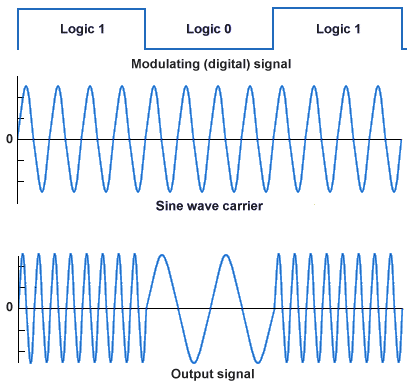
\includegraphics[scale = 0.4]{bfsk.png}
        \caption{Example of Binary FSK}
        \label{fig:m_label}
    \end{figure}
    $x_0(t)$ to represent 0 \\
    $x_1(t)$ to represent 1
\end{frame}

\begin{frame}{Theory}
    Let $s_0$ be the component of signal for 0 in the received signal \\
    Let $s_1$ be the component of signal for 1 in the received signal \\
    \bigbreak
    \textbf{Ideal case} \\
    \bigbreak
    \textit{For 0} \\
    $\begin{pmatrix}
        s_0 \\
        s_1
    \end{pmatrix} =
    \begin{pmatrix}
        \sqrt{A} \\
        0
    \end{pmatrix}$
    \bigbreak
    \textit{For 1} \\
    $\begin{pmatrix}
        s_0 \\
        s_1
    \end{pmatrix} =
    \begin{pmatrix}
        0 \\
        \sqrt{A} 
    \end{pmatrix}$
\end{frame}
    
\begin{frame}{}
    \begin{figure}
        \centering
        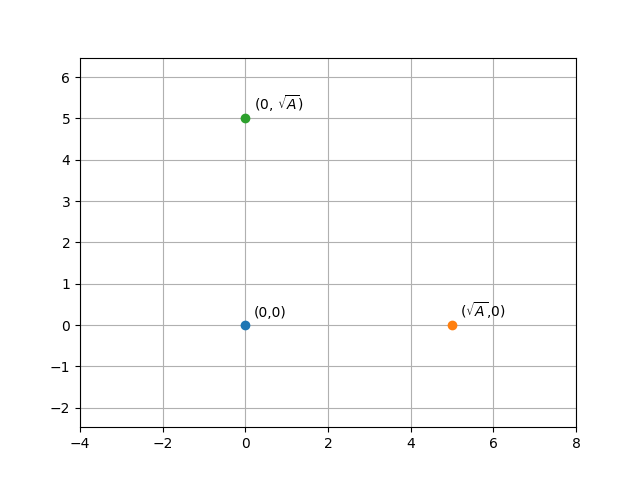
\includegraphics[scale = 0.5]{first.png}
        \caption{Ideal case}
        \label{fig:my_label}
    \end{figure}
\end{frame}

    
\begin{frame}{}
    But normally, the channel adds noise to the signal. \\ 
    Suppose the noise has the form of Additive White Gaussian Noise \\
    \[ \mathcal{N} (0, N)\] 
    \bigbreak 
    The received components can then be modelled as \\
    \[\textbf{y} = \textbf{s} + \begin{pmatrix} n_0 \\ n_1 \end{pmatrix}\]
    \bigbreak
    where $N_0$ and $N_1$ are also Gaussian with 0 mean and finite variance. \\
    Let us assume variance as 1 for convenience, i.e., 
    \[N_0, N_1 \sim \mathcal{N} (0, 1) \]
    \bigbreak
\end{frame}

\begin{frame}{}
    \textit{If 0 is sent} \\
    $\begin{pmatrix}
        y_0 \\
        y_1
    \end{pmatrix}$ =
    $\begin{pmatrix}
        \sqrt{A} + n_0 \\
        n_1
    \end{pmatrix}$
    \bigbreak
    \textit{If 1 is sent} \\
     $\begin{pmatrix}
        y_0 \\
        y_1
    \end{pmatrix}$ =
    $\begin{pmatrix}
        n_0 \\
        \sqrt{A} + n_1 
    \end{pmatrix}$
\end{frame}

\begin{frame}{Simulation}
    \begin{figure}
        \centering
        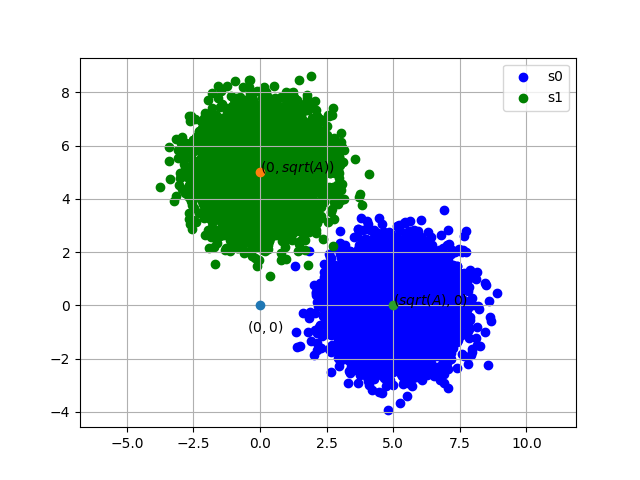
\includegraphics[scale = 0.5]{bfsk_scatter.png}
        \caption{Simulation after addition of noise, if 0 and 1 are equi-probable}
        \label{fig:my_label}
    \end{figure}
\end{frame}

\begin{frame}{Code}
    simlen = 1e4 \\
    a=5 \\
    \bigbreak
    s0 = np.array([1,0]) \\
    y0 = [((a*s0[j])+np.random.normal(0, 1, int(simlen))) for j in range(2)] \\
    \# y0 is 2 x simlen array = ( sqrt(A)+n1 , n2) \\
    \bigbreak
    s1 = np.array([0,1])
    y1 = [((a*s1[j])+np.random.normal(0, 1, int(simlen))) for j in range(2)] \\
    \# y1 is 2 x simlen array = ( n1 , sqrt(A)+n2)
\end{frame}

\begin{frame}{Guessing y}
    \begin{figure}{}
    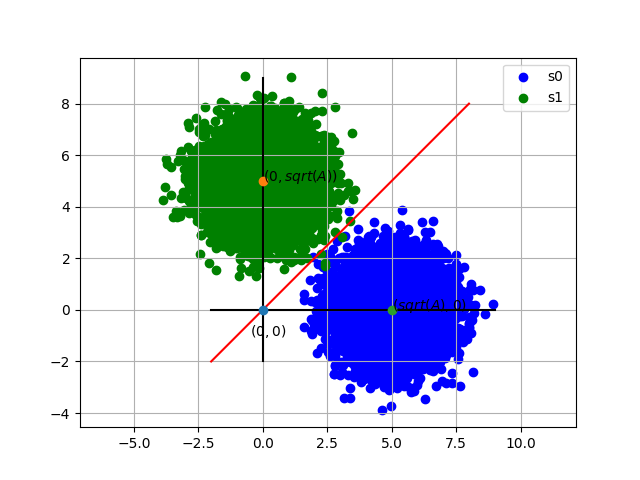
\includegraphics[scale=0.55]{bfsk_decision}
    \end{figure}
\end{frame}

\begin{frame}{Decision}
    \begin{block}{How do you guess s, i.e, $\hat{s} | $ 
    \mathbf{y}=?}
    If $|y-s_0| < |y-s_1| $, decide s=$s_0$,\\
    else, s = s_1\\
    \end{block}
\end{frame}

\begin{frame}{Mathematical Derivation}{}
\begin{block}{Multivariate Gaussian PDF}

\begin{multline}
p(x,y)= \frac{1}{2\pi \sigma_x\sigma_y\sqrt{1-\rho^2}}\exp\lsbrak{-\frac{1}{2\sqrt{1-\rho^2}}}
\\
\times \rsbrak{\cbrak{\frac{\brak{x-\mu_x}^2}{\sigma_x^2}+\frac{\brak{y-\mu_y}^2}{\sigma_y^2}-\frac{2\rho\brak{x-\mu_x}\brak{y-\mu_y}}{\sigma_x\sigma_y}}}
\end{multline}

\end{block}
 P(r$|s_o$)=P($r_1,r_2|s_o$)=P(\sqrt{A}+$n_1,n_2$)\\
Let \sqrt(A)=a\\

E($r_1)=E(a+n_1)=a+E(n_1)=a$ \\
E($r_2)=E(n_2)=E(n_2)=0$ \\

\end{frame}

\begin{frame}{cntd}
\sigma_{r_1}=\sigma_{a+n_1}=\sigma_{n_1}=\sigma \\
\sigma_{r_2}=\sigma_{n_2}=\sigma_{n_2}=\sigma\\
Substituting the above values keeping in mind n1,n2 are independent\\
we get \rho = 0

\begin{multline}
p(r|s0)= \frac{1}{2\pi \sigma^2}\exp\frac{-1}{2}\times \frac{\brak{r_1-a}^2}{\sigma^2}+\frac{\brak{r_2}^2}{\sigma^2}
\end{multline}
\end{frame}


\begin{frame}{Decision}
\begin{block}{Detecting s0}
P(s_0|r)>P(s_1|r)\\ Now apply Baye's conditional probility\\
\bigbreak
P(s_0)\frac{P(r|s_0)}{P(r)} >P(s_1) \frac{P(r|s_1)}{P(r)}\\
\bigbreak
If $s_0$ and $s_1 $ are equiprobable, the above expression reduces to\\
P($r|s_0$) $>$ P($r|s_1$)\\
\bigbreak
i.e, $-(r1-a)^2-r2^2 > -(r1)^2-(r2-a)^2$
\bigbreak
  $2r_1a > 2r_2a$
  \bigbreak
  
  $r_2<r_1$ for detecting s0
  
\end{block}
    
\end{frame}

\end{document}
